% LumenRadar — working LaTeX skeleton (v0.1)
% Compile: pdflatex paper.tex && bibtex paper && pdflatex paper.tex x2
% For submission: switch documentclass to IEEEtran (conference) — kept as
% plain article here so the skeleton compiles on minimal TeX installs.
\documentclass[10pt]{article}
\usepackage[a4paper, margin=2.5cm]{geometry}
\usepackage{amsmath, amssymb}
\usepackage{graphicx}
\usepackage{booktabs}
\usepackage{url}
\usepackage[numbers]{natbib}
\usepackage{xcolor}
\newcommand{\todo}[1]{\textcolor{red}{[TODO: #1]}}

\title{Detecting Covert Optical Signaling in Camera Footage:\\
A DSP Pipeline for Blink-Count and Brightness Channels}
\author{Samet Y{\i}lmaz Temel\\
0rce-Labs\\
\url{https://github.com/0rce-Labs/lumenradar}}
\date{October 2026 --- working draft}

\begin{document}
\maketitle

\begin{abstract}
Consumer software can modulate a screen or status LED so that a nearby camera
receives data a human supervisor misses: answer codes encoded as blink counts,
brightness pulses, or sub-perceptual luminance oscillation. The attack side of
this channel family is well studied; the \emph{detection} side is not --- prior
work explicitly leaves camera-based monitoring unimplemented. We present
LumenRadar, an open-source detector that analyzes ordinary video with a
three-detector DSP pipeline (narrow-band periodicity, burst pulse-count
structure, session-baseline comparison) fused with camera-artifact rejection
into an explainable verdict. On synthetic calibration through an mp4 codec
round-trip, the pipeline detects 2\,Hz modulation down to
$\sim$4 gray levels peak-to-peak at 30\,fps with zero false positives, and
recovers blink-count symbol sequences exactly. On a real-hardware screen-recording
dataset (Retina 2880$\times$1800, variable frame rate), all three positives are
detected with no false positives after three genuine real-world defects ---
screen-rendered beacons beyond LED-size heuristics, low-duty lead-in timing,
and VFR spectral leakage --- surfaced by the data and were fixed
\end{abstract}

\section{Introduction}
Screen- and LED-control software in the exam-proctoring evasion space now ships
covert answer channels: menu-bar icons, Caps-Lock LED blink counts, keyboard
backlight pulses, and screen-brightness flashes, marketed as undetectable in
video-conferencing proctoring. The optical covert-channel literature covers the
attack side extensively
\cite{leditgo2017,brightness2020,visisploit2016,hilight2016,receiver2023}, but
detection remains an open gap: \cite{brightness2020} explicitly describes
camera-based monitoring as ``nontrivial'' and leaves it unimplemented, while
receiver-side work solves \emph{decoding} --- the attacker's problem ---
not \emph{detection}.

This paper contributes:
\begin{enumerate}
  \item a three-detector DSP pipeline fused with artifact rejection into an
        explainable verdict (\S\ref{sec:method});
  \item the first open-source detector targeting blink-count symbol
        modulation in the proctoring context;
  \item a perceptibility-based calibration quantifying the detection floor
        ($\sim$4 gray levels p-p, 30\,fps, mp4 round-trip) and an
        open dataset protocol with integrity-hashed manifests
        (\S\ref{sec:dataset}).
\end{enumerate}
Scope: detection only. The accompanying repository contains no transmitter and
no answer-generation path; its calibration beacon exists solely to label
positive-class samples on the defender's own hardware.

\section{Related Work}
\begin{table}[h]
\centering
\small
\begin{tabular}{@{}llll@{}}
\toprule
Work & Channel & Direction & Gap we fill \\
\midrule
LED-it-GO \cite{leditgo2017} & HDD LED OOK, 4\,kbit/s & attack & tape/jam only \\
BRIGHTNESS \cite{brightness2020} & screen brightness & attack & detection ``nontrivial'' \\
VisiSploit \cite{visisploit2016} & sub-perceptual images & attack & --- \\
HiLight \cite{hilight2016} & translucency FSK & attack (decode) & DSP adapted defensively \\
Sensors'23 \cite{receiver2023} & brightness 2-PAM & attack (decode) & decoding $\neq$ detecting \\
\bottomrule
\end{tabular}
\caption{Positioning against the optical covert-channel literature.}
\label{tab:related}
\end{table}

\section{Threat Model}
\textbf{Attacker:} an app or malware controlling an LED or screen region on the
supervised device, plus a receiver camera with line of sight.
\textbf{Defender:} holds only a camera stream (e.g.\ the proctor webcam); no
access to the supervised device. \textbf{Signal classes:} (1) blink-count
symbols (1--4 pulses $=$ choice A--D, repeated), (2) periodic brightness
pulses, (3) sub-perceptual narrowband oscillation. PWM-rate channels beyond
camera Nyquist are out of scope.

\section{Method}\label{sec:method}
Per clip: ingest $\rightarrow$ LED ROI localization (small saturated stable
blob; manual override; full-frame fallback) $\rightarrow$ ROI luminance series
plus a control series (frame mean with the ROI/ring excluded) $\rightarrow$
three detectors $\rightarrow$ artifact classification $\rightarrow$ fused
verdict with full evidence.

\textbf{M1 --- band periodicity (0.5--15\,Hz).} Hann PSD with three gates:
absolute amplitude $A = 4\sqrt{P}/N \ge 0.5$ gray (perceptibility; also kills
out-of-band leakage skirts), peak-to-local-floor ratio $\ge 8$, and peak above
the Gumbel noise-max expectation $2(\ln n + \gamma)$. Harmonic confirmation
against the global floor.

\textbf{M2 --- burst pulse-count.} Threshold segmentation $\rightarrow$
intervals $\rightarrow$ bimodal split at the largest jump (a median split
collapses when single-count symbols dominate) $\rightarrow$ symbol counts;
detected iff counts repeat AND intra-gap CV $\le 0.6$ AND inter-gap CV
$\le 0.35$ AND gap contrast $\ge 2$. Aperiodic activity (e.g.\ HDD LEDs)
fails the pacing test.

\textbf{M3 --- session baseline.} The first 2\,s form a beacon-free profile;
candidate windows are compared by smoothed PSD ratio with
$z \ge 5$ (log-ratio $\sigma=\sqrt{2\psi'(5)}$) AND amplitude
$\ge 0.5$ gray --- near-zero-energy baselines make raw ratios explode on
codec/quantization noise.

\textbf{Artifacts.} Auto-exposure hunting: ROI/control lockstep
($r \ge 0.85$) \emph{with} comparable magnitude (control/ROI std $\ge 0.25$);
correlation alone is fooled by mp4 block-coupling (measured
$r = 0.86$--$0.98$ with $\approx 0$ control amplitude). Mains $2f$ aliases are
flagged only when Nyquist covers 100/120\,Hz. Full-frame mode derives a spatial
control from the border ring.

\section{Dataset Protocol}\label{sec:dataset}
Clips follow a \texttt{pos\_/neg\_} naming contract; a SHA-256 manifest pins
integrity; the evaluator runs the identical analysis path as the CLI.
Real-hardware results (6 clips: 3 positives, 3 negatives, Retina 2880$\times$1800
screen recording, 24--52\,fps VFR): \textbf{3/3 positives detected}
(2$\times$\textsf{signal\_detected} as \textsf{blink\_count} with symbol
intervals recovered, 1$\times$\textsf{suspicious} \textsf{periodic} at the true
1.8\,Hz), \textbf{0 false positives}. Capturing these numbers surfaced three
real-world defects that synthetic data alone could not: the calibration beacon
renders as a $\sim$300\,px solid bright square beyond the small-LED ROI
heuristic (fixed with a class-aware beacon-square scan), low-duty blink
patterns need a wider ROI probe window (first ON frame at 0.65\,s), and
variable-frame-rate capture turns a strong tone's spectral skirt wide enough
to defeat local-floor ratios (fixed with a strong-amplitude$+{}$harmonic
bypass, and a sustained-power gate that rejects step-edge transients ---
measured 0.05 vs 1.00 sustained-fraction separation). Real-hardware recordings
are not redistributed; a SHA-256 manifest and all generation/analysis scripts
are provided for independent verification, and clips are available from the
author on reasonable request (see \texttt{docs/DATASET-POLICY.md}). Remaining
for the journal version: scaled-up dataset (2 devices $\times$ 3 lighting,
$\ge$60 clips) and formal ROC.

\section{Synthetic Calibration (preliminary)}
Config: 30\,fps, 6\,s clips, structured background scene, 16$\times$16 LED,
mp4v round-trip, 5 seeds per amplitude, 10 clean seeds. Detection floor
(2\,Hz sine, TPR $5/5$ from): \textbf{4 gray levels p-p}; clean FPR
\textbf{0/10}. Frequency sweep ($\sim$76 gray levels p-p, 3 seeds/frequency):
TPR $3/3$ at every frequency from 0.5 to 14\,Hz with the peak recovered at the
true frequency; at 15\,Hz the mp4 codec itself destroys the signal (amplitude
drops to $\approx$0.1 gray), so the practical band edge is codec-bound, not
detector-bound. End-to-end: clean/noisy $\rightarrow$ clean; blink pattern
$(1,1,2,1,2,\dots)$ $\rightarrow$ \textsf{signal\_detected} with symbol counts
recovered exactly after codec; whole-frame oscillation $\rightarrow$
\textsf{camera\_artifact}. Runtime: $\sim$12--16$\times$ realtime on an
ARM aarch64 core (30\,s clip in 2.2\,s). All numbers are synthetic-only;
real-camera data are expected to shift the floor.

\begin{figure}[h]
\centering
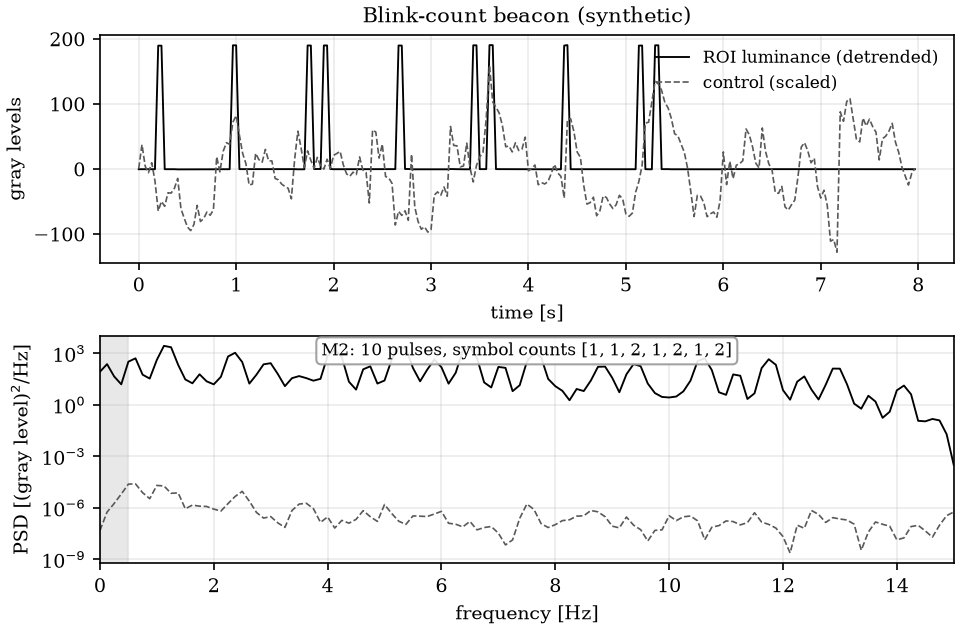
\includegraphics[width=\linewidth]{figures/fig_burst.png}
\caption{Blink-count beacon (synthetic, codec round-trip). Top: detrended ROI
luminance (black; 10 pulses in symbol groups) vs.\ the ROI-excluded control
(dashed gray, scaled). Bottom: Welch PSD of both channels; the shaded strip is
the excluded $<0.5$\,Hz band. The annotation reports the M2 detector output:
10 pulses, symbol counts $[1,1,2,1,2,1,2]$ --- recovered exactly through the
codec.}
\label{fig:burst}
\end{figure}

\begin{figure}[h]
\centering
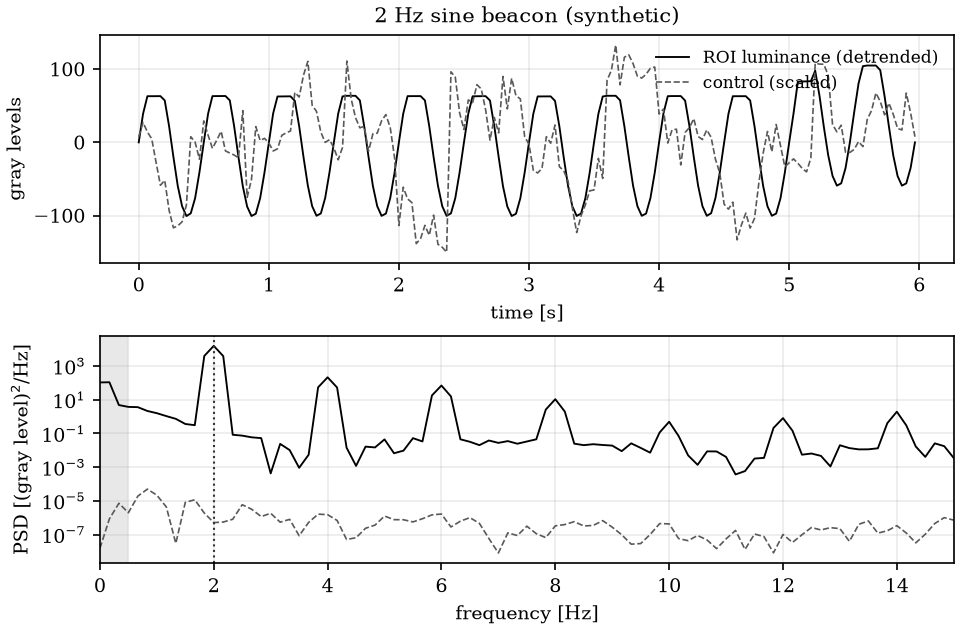
\includegraphics[width=\linewidth]{figures/fig_periodic.png}
\caption{Narrowband beacon (synthetic): 2\,Hz modulation is $\sim$8 orders of
magnitude above the control channel in the Welch PSD; the dotted marker is the
M1 peak.}
\label{fig:periodic}
\end{figure}

\section{Countermeasures}
For flagged sessions: physical LED-covering policy, brightness-locked displays,
proctor-cam exposure lock, and continuous session-baseline monitoring. Detector
output is evidence (JSON), never an automated accusation.

\section{Threats to Validity}
Synthetic scenes lack realistic illumination dynamics; the beacon is
machine-timed while human-driven codes jitter (M2 CV thresholds may need
loosening); adaptive adversaries can randomize duty cycles to defeat pacing;
lossy webcams compress away sub-0.5-gray signals --- which also raises the
attacker's required modulation depth, favoring the defender.

\section{Conclusion and Roadmap}
LumenRadar closes a documented gap: an open, explainable detector for covert
optical signaling in ordinary camera footage, with a calibrated synthetic
floor and a reproducible dataset pipeline. Next: real-hardware ROC, arXiv
preprint, conference submission.

\bibliographystyle{unsrtnat}
\bibliography{refs}

\end{document}
